\documentclass{IEEEtran}

\usepackage{ifthen}
\usepackage[normalem]{ulem} % for \sout
\usepackage{xcolor}
\usepackage{amssymb}
\newcommand{\ra}{$\rightarrow$}
\newboolean{showedits}
\setboolean{showedits}{true} % toggle to show or hide edits
% \setboolean{showedits}{false} % toggle to show or hide edits
\ifthenelse{\boolean{showedits}}
{
	\newcommand{\ugh}[1]{\textcolor{red}{\uwave{#1}}} % please rephrase
	\newcommand{\ins}[1]{\textcolor{blue}{\uline{#1}}} % please insert
	\newcommand{\del}[1]{\textcolor{red}{\sout{#1}}} % please delete
	\newcommand{\chg}[2]{\textcolor{red}{\sout{#1}}{\ra}\textcolor{blue}{\uline{#2}}} % please change
}{
	\newcommand{\ugh}[1]{#1} % please rephrase
	\newcommand{\ins}[1]{#1} % please insert
	\newcommand{\del}[1]{} % please delete
	\newcommand{\chg}[2]{#2}
}

\newboolean{showcomments}
\setboolean{showcomments}{true}
% \setboolean{showcomments}{false}
\newcommand{\id}[1]{$-$Id: scgPaper.tex 32478 2010-04-29 09:11:32Z oscar $-$}
\newcommand{\yellowbox}[1]{\fcolorbox{gray}{yellow}{\bfseries\sffamily\scriptsize#1}}
\newcommand{\triangles}[1]{{\sf\small$\blacktriangleright$\textit{#1}$\blacktriangleleft$}}
\ifthenelse{\boolean{showcomments}}
%{\newcommand{\nb}[2]{{\yellowbox{#1}\triangles{#2}}}
{\newcommand{\nbc}[3]{
 {\colorbox{#3}{\bfseries\sffamily\scriptsize\textcolor{white}{#1}}}
 {\textcolor{#3}{\sf\small$\blacktriangleright$\textit{#2}$\blacktriangleleft$}}}
 \newcommand{\version}{\emph{\scriptsize\id}}}
{\newcommand{\nbc}[3]{}
 \renewcommand{\ugh}[1]{#1} % please rephrase
 \renewcommand{\ins}[1]{#1} % please insert
 \renewcommand{\del}[1]{} % please delete
 \renewcommand{\chg}[2]{#2} % please change
 \newcommand{\version}{}}
\newcommand{\nb}[2]{\nbc{#1}{#2}{orange}}

\definecolor{ibcolor}{rgb}{0.4,0.6,0.2}
\definecolor{ascolor}{rgb}{0,0.5,0.9}

\definecolor{bocolor}{rgb}{0.6,0.9,0.2}
\definecolor{jrcolor}{rgb}{0.5,0,0.5}
\definecolor{hkcolor}{rgb}{0.4,0.1,0}
\definecolor{nrcolor}{rgb}{1.0,0.6,0.1}
\definecolor{tdcolor}{rgb}{1.0,0,0}

\newcommand\ivan[1]{\nbc{IB}{#1}{ibcolor}}
\newcommand\arsj[1]{\nbc{AS}{#1}{ascolor}}
\newcommand\nsr[1]{\nbc{NSR}{#1}{nrcolor}}
\newcommand\jr[1]{\nbc{JR}{#1}{jrcolor}}
\newcommand\bo[1]{\nbc{BO}{#1}{bocolor}}
\newcommand\hk[1]{\nbc{HK}{#1}{hkcolor}}
\newcommand\todo[1]{\nbc{TODO}{#1}{tdcolor}}


\usepackage{booktabs} % For formal tables

\usepackage[pdftex]{graphicx}
\usepackage[shortcuts,acronym]{glossaries}
\usepackage{listings}
\usepackage[ruled]{algorithm2e} % For algorithms
\usepackage[draft]{hyperref} % draft remove all hyperlinks
\usepackage{verbatim}
\usepackage{float}


\renewcommand{\algorithmcfname}{ALGORITHM}
\SetAlFnt{\small}
\SetAlCapFnt{\small}
\SetAlCapNameFnt{\small}
\SetAlCapHSkip{0pt}
\IncMargin{-\parindent}

\renewcommand{\lstlistingname}{Code}% Listing -> Algorithm

%\newacronym{mba}{MBA}{Microservice-Based Application}
\newacronym{soa}{SOA}{Service-Oriented Architecture}
\newacronym{mvc}{MVC}{Model-view-controller}

\newcommand\el{\emph}

\IEEEoverridecommandlockouts

% Document starts
\begin{document}
%
%
%%\title{Uncovering Microservice Dependencies \\ to Support Maintenance and Evolution}
%%\title{Uncovering Microservice Dependencies \\ to Support Evolution}
\title{EnergyMAC : A Framework for User-centric Energy Control}
%
%
\author{
  \IEEEauthorblockN{
           Harsha and
           Satish
   }
%%    \and
%%    \and
%%        \IEEEauthorblockA{
%%                \IEEEauthorrefmark{1}Federal University of Pernambuco, Brazil %\\
%%                    %\{arsj2,nsr\}@cin.ufpe.br    
%%        }
%%        \and
%%        \IEEEauthorblockA{             
%%                \IEEEauthorrefmark{4}University of British Columbia, Canada %\\
%%                    %devkhv129@gmail.com \\
%%                    %\{bo,mjulia\}@ece.ubc.ca \\
%%                    %bestchai@cs.ubc.ca
%%        }
%%        \and
%%        \IEEEauthorblockA{
%%               \IEEEauthorrefmark{2}IBM, Canada  %\\
%%        }
%%        \and
%%        \IEEEauthorblockA{
%%               \IEEEauthorrefmark{3}IBM, USA  %\\
%%                   %jstein@ca.ibm.com\\
%%                   %aerwin@us.ibm.com                  
%%        }   
}
%
\maketitle
%
%%%%%%%%%%%%%%%%%%%
%\begin{abstract}
%%Smartphones are increasingly becoming an important part of our life. With a limited battery capacity in smartphones, energy efficiency is an important requirement for good android applications. Applications in a smartphone can have varying degrees of importance for android user. For example, healthcare apps tied to a smartwatch and financial apps which report real-time market updates may be more critical and important to users than mobile games. In the current Android system, there is no feature for user to give more importance for energy usage of certain apps over other. To address this, in this project, we implemented an EnergyMAC framework which enables users to prioritize energy for high priority applications installed on their smartphones. 
%\end{abstract}

%%%%%%%%%%%%%%%%%%%
%
%
%% The default list of authors is too long for headers}
%%\renewcommand{\shortauthors}{G. Zhou et al.}
%
%%%%%%%%%%%%%%%%%%%%%%%%%%%%%%%%%%%%%%%%%%%%%%%%%
\section{Introduction}
\label{intro}
%%%%%%%%%%%%%%%%%%%%%%%%%%%%%%%%%%%%%%%%%%%%%%%%

Microservices ~\cite{DBLP:journals/corr/DragoniGLMMMS16} a new trend in architecting large software systems wherein a system is designed as a set of microservices. Microservices can be developed, managed and scaled independently. There is typically some kind of routing fabric ~\cite{Selimi:2017:PSP:3101112.3101167} that gets requests to a specific instance of a microservices; this routing fabric often provides load-balancing and can isolate microservices that are in a failed state. There are costs to this approach as well such as the computational overhead of running an application in different processes and having to pay network communication costs ~\cite{7742218} rather than simply making function calls within a process.

Using Web standards is recognized as a common approach in building microservices application architectures. REST mechanism is widely used for data-interchange ~\cite{DBLP:journals/corr/DragoniGLMMMS16} in microservices. It is a useful integration method because of its comparatively lower complexity over other protocols. Some of the basic properties of a REST protocol is statelessness and cache-ability. These properties will facilitate performance and reliability improvements in applications using REST.

For an efficient communication between microservices using REST, we need certain basic services like name-resolution of service endpoints, load balancing between different instances of the same service and caching of REST objects. Currently, these services are not provided by the network, But they are provided by external systems like DNS and middleboxes like HTTP cache. This middleware can introduce extra latency to API call under certain conditions such as cache miss event.  

The Named Data Networking (NDN) ~\cite{zhang2014named} project aims to develop a new Internet architecture that can capitalize on strengths and address weaknesses of the Internet’s current host-based, point-to-point communication architecture in order to naturally accommodate emerging patterns of communication. By naming data instead of their locations, NDN transforms data into a first-class entity. It also enables several radically scalable communication mechanisms such as automatic caching to optimize bandwidth.

In this project, we will apply NDN features like named routing and automatic caching using in-network storage to create a REST implementation on NDN without middleboxes that can introduce latencies. We will evaluate our implementation by showing the reduced end-to-end latency of a REST API in our sample microservices application.

In section ~\ref{related}, we will introduce to existing solutions and NDN architecture. In section ~\ref{motivation}, we will give problem statement and motivation for the problem. Section ~\ref{solution} will contain a description of the proposed solution. Finally, in ~\ref{evaluation}, we will specify our evaluation strategy. 




%\input{dependencies}
%%%%%%%%%%%%%%%%%%%%%%%%%%%%%%%%%%%%%%%%%
%\vspace{0.1in}
\section{Related work}
\label{related}
%%%%%%%%%%%%%%%%%%%%%%%%%%%%%%%%%%%%%%%%
\subsection{Existing solutions for service discovery}

There are multiple solutions for service discovery in microservices. The simplest solution to registration and discovery is to just put all of the service endpoints belonging to a microservice behind a single DNS name ~\cite{cheshire2013dns}. To address a service, we can contact it by DNS name and the request should get to a random back-end hosting the microservice. Main drawbacks of this approach are DNS suffers from propagation delays; even after a server failure is detected a de-registration command issued to DNS, there will be at least a few seconds before this information gets to the consumers. Also, due to the various layers of caching in the DNS infrastructure, the exact propagation delay is often non-deterministic. Another major problem is that a service is identified just by name, there is no way to determine which boxes get traffic. We will get the equivalent of random routing, with loads chaotically piling up behind some back-ends while others are left idle. 

In contrast to DNS based approach, our NDN based service discovery can load balance the flows ~\cite{tan2016flow} among different instances of the same microservice at the NDN router. It has faster recovery from service failures. As soon as NDN router identify service failures; it will invalidate the link. if a new request comes to the same service our NDN router will simply use alternate path for propagation. 

Etcd ~\cite{etcd} is a key-value store that provides shared configuration and service discovery for Container Linux clusters. etcd runs on each node trying to form a cluster using Raft ~\cite{raft} with the others for achieving high availability and fault-tolerance. It also supports service reconfiguration by watching updates to key prefixes with the service name. Another work is Consul ~\cite{Consul} that provide consistent key-value store to deliver service discovery and integrated health checking based Consul agents. These agents communicate with Consul servers where data is stored and replicated, to maintain cluster state. Synapse ~\cite{Synapse} is a system for service discovery
whose heart is a HAProxy, a stable and proven routing component. Synapse runs the HAProxy on application servers that are used to route requests from application servers to service providers running in the cluster. In order to provide service discovery, Synapse comes with several watchers, which frequently check for changes to the service location to update the
HAProxy configuration. Docker Swarm ~\cite{swarm} is a native cluster system for Docker hosts. Docker Swarm decides where service images should be deployed to, thus each Swarm needs a key-value store which acts as a DNS server to store the location of each service. Each host has a Swarm agent running which is responsible for advertising its attributes to the key-value store.

Above-mentioned solutions use a consistent key-value store that is mainly achieved through cluster implementation. In practice, service discovery mechanisms that use the cluster to preserve the system reliability adds complexity to deployments. With the solutions that form a quorum to maintain cluster’s activities strongly depend on the number of servers. Without a sufficient number of cluster nodes, the server nodes cannot
form a Raft-based quorum, thus the cluster cannot operate, and data loss can occur. Moreover, these solutions might occur high event advertising overhead for synchronizing the service state on every cluster nodes. Furthermore, there would be a significant increment of service records due to the number of available service instances. Therefore, it is very difficult to scale when applications have larger service popularity or
applications grow larger.

%\input{exampleApp}
%%%%%%%%%%%%%%%%%%%%%%%%%%%%%%%%%%%%%%%%%%%%%%%%
\section{Problem}
\label{motivation}
%%%%%%%%%%%%%%%%%%%%%%%%%%%%%%%%%%%%%%%%%%%%%%%%


%Why we are building this system - motivation
One of the main requirements for an Android application is energy efficiency. Current energy management techniques in android give a little scope for energy control of applications based on user preferences. In this project, we develop a framework based on Android to enable user-centric energy management. This framework will enable users to give priority to the energy consumption of apps that are of high value to them. Furthermore, it will also give incentive for developers to create applications that are energy efficient. 


%Who are stake holders and what they want
There are three stakeholders that are mainly affected by this framework

\begin{enumerate}

\item Android end users
\item Android App developers
\item Smartphone device manufactures

\end{enumerate}

%What we are building
Users have a limited power in their Smartphone batteries. Among many applications installed by a user on their Smartphone, only a few frequently used applications are more important for them. For a user who is mindful of his battery life may want to restrict applications that have a high energy usage but has a little value for the user. To restrict such apps from consuming all of the energy, a user can use our framework to provide a priority for each app installed on their Smartphone. A user can give either high, medium, or low priorities for an app based on their preference. By default, applications will be in low priority when they are initially installed in the phone. 

High priority applications and the Android operating system itself are considered to be most important applications for the user and are allowed to unrestricted use of the energy. Energy usage of medium and low priority applications are considered to be less important for the user and energy usage of these applications are restricted by our framework. 

Android application developers should adapt their lower priority applications to make them more energy efficient. Energy used by applications will be accounted for and certain system resources will be denied when they use more energy than allowed by its priority. Application developers should accommodate these new insufficient energy errors and build their app accordingly to work for low, medium and high priorities. Some of the current applications such as Facebook have both full-fledged and lite applications for different kinds of phones and networks.

Accurate energy accounting depends on specific device and battery used. Hence the framework should be customizable for device manufacturers so that they can optimize for their devices and battery type used. 


%What are constriants of our system
Keeping various stakeholders in mind, our system should always ensure following properties

\begin{enumerate}
\item Always higher priority applications can use more energy than a lower priority application.
\item Fairness among all applications belonging to same priority should be ensured.
\item The system should consider the changes in total available energy as the battery drains over the time.
\item It should also take into account for changes in the number of energy consumers that are active in the Smartphone. 
\item The framework should have minimal overhead.
\item The framework should ensure failures due to lack of energy are graceful and developers are notified.
\item The framework shouldn't reclaim energy once allocated to an app unless application releases or gets killed. 
\item Apps should benefit when system gains energy due to recharge of battery.
\item The system should be customizable for different hardware devices and battery.

\end{enumerate}


In the next section, we will look at how system is designed to satisfy these properties.


\section{Solution}



\subsection{System design}


In this section, we will introduce fundamental unit of measurement for energy in our system, how we account for energy consumption of applications and finally how we will allocate energy between applications to ensure system properties are met.

\subsection{Unit of measurement}

An abstract unit of energy in our system is called energy credit. Having an abstracted unit will help us to make the framework more customizable for Android device makers. By default, an energy credit is equivalent to 1 mAh in the current prototype implementation. When a resource of an Android system such as the network or the disk is used by an application, it will spend some energy credits equivalent to the amount of energy spent in executing that system functionality.

\subsection{Energy accounting for system resources }

Android uses Linux kernel to manage system resources. In Linux kernel, system calls are the single point of contact for all user-level applications. Any user functionality that requires system resources such as network can only be executed by calling corresponding system calls. Using this fact, there are many previous android energy modeling techniques such as Eprof, which can calculate the energy consumption for each system call. In our framework, we will estimate amount of energy required to execute a system call and allow system call to execute only when required energy for application is available.

System calls can have either constant or varying energy cost. System calls such as socket::connect has a constant energy cost and socket::send has an energy cost depending on the amount of data it needs to send. Constant cost system calls can be estimated before hand and can be stored in a hash table. Verifying system calls with dynamic cost require a model to predict cost based some variables such as amount of data to be transfered as in the case of socket::send. These models can be different for different devices, we can create these models using values estimated using Eprof based on different parameters.

\subsection{ Allocation of credits }

Energy credit allocation among applications in a dynamic system such as Android can be tricky. The total number of available energy credits change as the battery is discharged continuously. Number applications consuming energy will also change with time. Furthermore, some applications will only be installed in the system, but may never be used. Hence it's important to carefully allocate energy credits to ensure all of the system properties stated in the section ~\cite{motivation}  are met.

The lithium-ion batteries used in modern Smartphones have the capacity range from 1000 mAh to 5000mAh. For example, If a phone is fully charged and the battery has a capacity of 2000mAh and if applications has a continuous load of 200 mA, then the battery will last for 10 hours. By decreasing load on the battery, we can decrease overall power consumption and increase battery life. In the previous example, if applications only has a load of 100 mA then the battery will last for 20 hours.  To facilitate this we need to limit the amount of energy spent by applications. In our framework, we will limit number energy credits an low priority application can spend in a time period. In the prototype implementation, we had the time period as 1 min.

Our system should limit energy consumption of low and medium android applications without affecting the energy consumption of the system and high priority applications. To ensure this, we will allocate an infinite number of credits for high priority and system apps. For medium and low priority applications, we will allocate 0.1\% and 0.05\% of total available credits respectively per time period. 

\subsection{Example}
Below is the example on how it will work
%Example 
Battery capacity is measured in Milli-Ampiers per hour. Normal smart phone battery will have 2000 mAh as capacity for fully charged battery. If operations as specified in Pathak et al. 



\subsection{How we met system properties}

\begin{enumerate}

%How will ensure system properties are meet

\item  This system will ensure that lower priority applications always has limited energy usage. This will force applications developers to create applications to have a minimal energy consumption. 

\item  It will always allocate applications with same priority same amount of energy credits.

\item  Rate is proportional to amount of battery available 

\end{enumerate}

\subsection{Limitations}

\begin{enumerate}

\item  The number of credits required for a system call is approximation of original value.
\item  Battery characteristics such as charge will change over the lifetime of the battery. 
\item  Certain existing operations which require high energy may fail.
\item  In cases such as tail energy applications can have energy impact without calling system calls.

\end{enumerate}

\subsection{Assumptions}

Following are assumptions we make in the Android system
\begin{enumerate}

\item  We account for all energy consumption with system calls.
\item  Apps either run in background or foreground are considered active and consume energy.
\item  Inactive apps don't consume energy.
\item  The total amount of available energy is constant for the time period.

\end{enumerate}





















\section{Implementation}\label{solution}

\begin{figure}[t]
%\vspace{0.2in}
\centering
%\resizebox{0.7\linewidth}{!}{
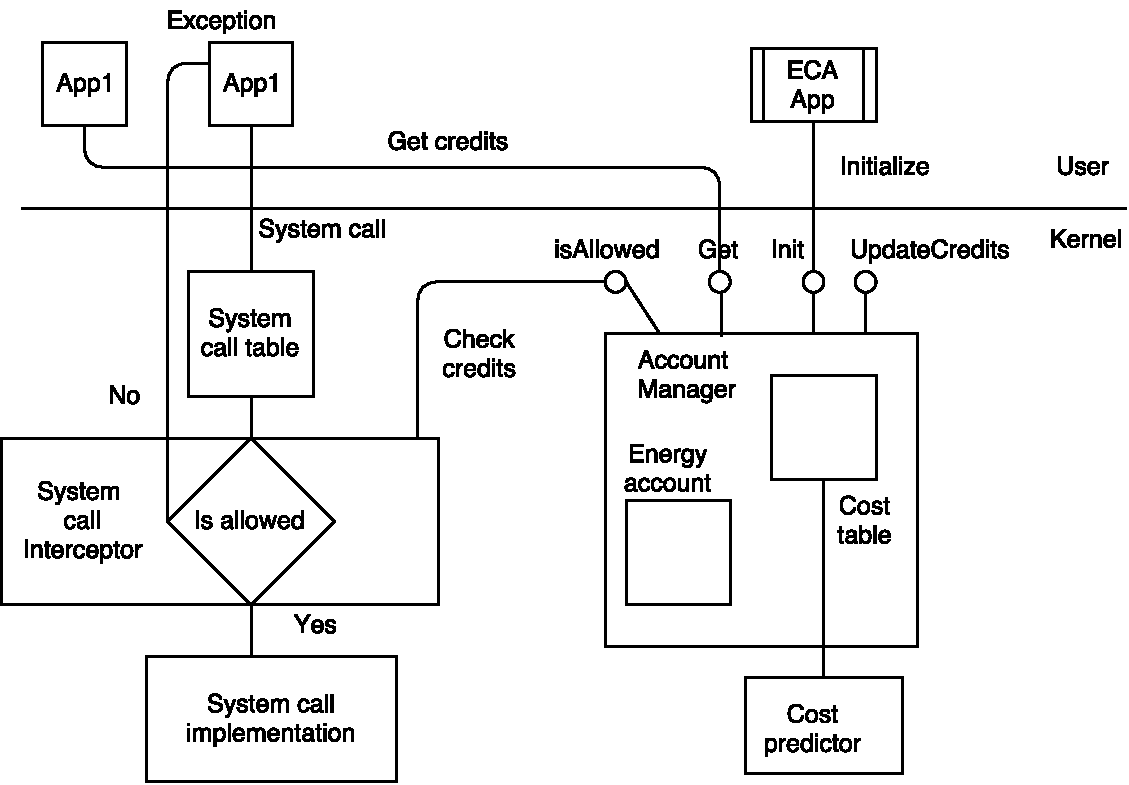
\includegraphics[width=0.8\linewidth]{Figs/mobileapp}
%}
\caption{Architecture.}
\label{fig:Architecture}
\centering
\end{figure}


\subsection{Technical Approach}

Our EnergyMAC framework (see Fig ~\ref{fig:Architecture}) comprises of four components:

\begin{enumerate}

\item Energy Credits allocation System App (ECA app): is a system app that facilitates user to see and allocate priorities for user apps installed in the mobile device. When a user allocates the priorities for apps, ECA app invokes the system call of Energy Accounting Manager in android kernel to save the app details and designated credits.

\item System Call Interceptor: is a component that intercepts the system calls from apps and consults Energy Accounting Manager to check credits that will be spent for that System Call and credits remaining for the app. If the enough energy credit is available, then it redirects to the actual system call else custom exception is thrown stating that required energy credits are not available for that operation.

\item Energy Accounting Manager: Two hash tables for storing records related to app's priority, assigned credits, and each System call's estimated cost (constant cost) are created in the Kernel. One table i.e. Energy account, is used for storing the app UID, priority and assigned credits and another table named Cost sheet is used for storing System call info and corresponding constant cost in terms of credits. Energy account will be refilled with credits at the end of each time period using a Linux kernel timer.

Energy Accounting Manager has access to above tables and exposes APIs for various operations:

\begin{itemize}
\item Get priority and length of time period for app/s
\item Update priority for app/s
\item Get cost of system call
\item Update cost of system call
\item Check if a given system call is allowed
\end{itemize}


\item System Call Price Manager: initializes cost table with cost for all system calls that have constant cost. Moreover, it will also estimate cost of variable cost system calls using models. These models will be derived from previous work such as Eprof.


\end{enumerate}

\subsection{How it works}

Android OS is divided between User Space and Kernel Space based on the type of actions that can be performed by user program and OS itself. This separation is required to provide isolation and abstraction. The Kernel has the privileges for managing the system resources and User programs do not. So, user program communicate with Kernel via system call to use services provided by OS. 

Each system call is represented by a number in system call table in the kernel. Since apps in the user space invoke system call for different operations, this system call can be intercepted and decision can be taken whether the system call should be executed. This is the basis for enforcing the energy accounting policies on apps in our energy accounting system. 

In Energy accounting system, the user allocates the available priorities for the apps that user intends to use via ECA App. This internally invokes the custom system calls that are part of Energy Accounting Manager, to update the priority of the apps and data is stored in the Energy account hash table. The accounting system had a kernel timer which times out at the end of each time period and credits will be updated in Energy account hash-table based on the priority of the app for next time period. 

The cost of each system call in terms of energy credits is decided by the System Call Price Manager depending upon the energy model for that system call and constant costs will be stored in the hash table named Cost sheet. 

When an app, in this case, GPS App, tries to use get the location, then it invokes the system call to get the location of the device. At this time, the system call is intercepted by the Interceptor and it checks with the Energy Accounting Manager if an app has enough credits to actually invoke that system call related to GPS. If the app has credits more than required to invoke the system call, then the Interceptor redirects to the actual system call and the corresponding credits for that system call is deducted from the allocated credits for that app. Otherwise, the custom exception is thrown back to the application stating that not enough credit is available for that operation and app has to adapt itself accordingly. 

The app can also check whether the operation is permitted and also time period with Energy Accounting Manager and change App's behavior accordingly. 



\subsection{Implementation choices}

There are mainly 5 different layers in Android OS i.e. System Apps, Java API framework, Native Libraries and Android Run time, Hardware Abstraction Layer and Linux Kernel. The Energy Accounting system could have been part of any layer but the decision to make it part of Kernel for the following reasons:

\begin{enumerate}

\item The operations will be protected: The malicious apps will not be able to steal the energy credits or change priority of other benign apps. Only System app and kernel components will have access to the system call related to energy credits update APIs.

\item If it were pushed to any layer above kernel, that would have involved changes in multiple components in that layer and it would not have been easily extendibles for future changes. The kernel is the centralized place to receive all the system calls and due this the changes required in one place and less invasive. For example if this energy accounting were to be moved to the Java API framework level, closer to the layer where app reside, then the changes had to be done in multiple components like Location Manager, Telephony manager,etc in this layer and that would have been more invasive.

\item Previous work such as Eprof has models for calculating energy costs of system calls. 

\end{enumerate}

Following changes were made in OS Kernel as part of the implementation:

\begin{enumerate}

\item System calls and their implementation corresponding to the APIs of the Energy Accounting Manager were added to the Kernel.
\item Two hash tables were created in the kernel memory to store energy accounting related information.
\item The system call number of the GPS system call i.e. sys ioctl was replaced by the system call number of the Interceptor in the system call table in the kernel.

\end{enumerate}




%\section{Evaluation}\label{evaluation}
In this section, we evaluate the performance overhead due to the control mechanism we have implemented in android kernel. In our experimental set up, we use original  and modified Goldfish Kernel on a emulator on a Linux machine for testing. 

\subsection{Experimental Goal}
Our idea focuses on  giving the control to  user on how the energy will be spent by different apps installed on the mobile phone. So, it becomes equally important to check and make sure that user does not see major performance hit in the system while using. The end goal of this experiment is to obtain performance overhead in terms of time introduced due to our changes.


\subsection{Methodology}
\begin{figure}[t]
	%\vspace{0.2in}
	\centering
	%\resizebox{0.7\linewidth}{!}{
	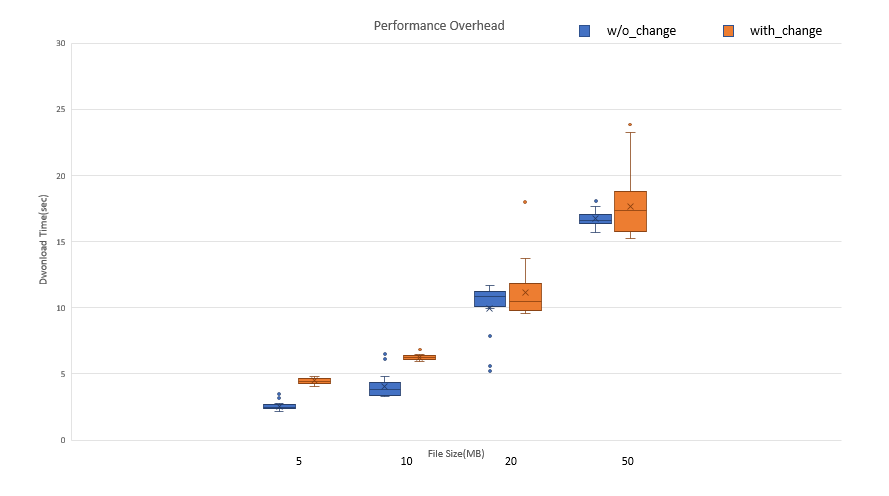
\includegraphics[width=\linewidth]{Figs/boxplot}
	%}
	\caption{Results for file downloads}
	\label{fig:result}
	\centering
\end{figure}

We developed a simple android app using which a user has options to download files of different sizes. In our experiment, we download a file of size 5 MB 20 times from server[https://www.thinkbroadband.com/download]and this is repeated for files of other sizes i.e. 10MB, 20MB, 50MB one after another from same server using our custom android app on the Android emulator. This experiment is conducted for two cases when (i) Emulator is running original/unmodified Goldfish kernel  (ii) Emulator is running Goldfish kernel with our modifications for control mechanism. 

%% figure here 
\subsection{Results}
We conducted evaluation by running the experiment 20 times for each file size as mentioned in the previous section and recorded the time taken for download and plot the data collected from the experiment. Figure ~\ref{fig:result} presents our experimental results. From this figure, it can be noted that mean overhead due to our modification is minimum i.e. under 2 seconds and this overhead would less likely to be visible to the user. Ideally, the overhead due to our modifications should remain constant as the operations of validating and updating the energy credits in the kernel layer for the apps remain same but the results show that it varies. This variation for each file size can be attributed to the fluctuations in download speed and network traffic.

In future, we plan to experiment using other user activity which is least affected by network fluctuations or any other factors.




%%%%%%%%%%%%%%%%%%%%%%%%%%%%%%%%%%%%%%%%%%%%%%%%%%
\section{Conclusion}
\label{conclusion}
%%%%%%%%%%%%%%%%%%%%%%%%%%%%%%%%%%%%%%%%%%%%%%%%

% originally on section model
%\begin{figure*}
  %  \centering
  %  \includegraphics[width=.8\textwidth]{figs/metamodel}
  %  \caption{Service evolution model.}
  %  \label{fig:metamodel}
%\end{figure*}


% example of citation ~\cite{Newman:2015}
%,Nadareishvili:2016} 

% example of a reference to other Section~\ref{sec:usecases}



%\bibliographystyle{IEEEtran}
%\bibliography{00}

\end{document}
